% IEEE GCCE 2026 -- 2-page submission (A4)
\documentclass[a4paper,conference,10pt]{IEEEtran}
\usepackage{graphicx}
\usepackage{url}
\usepackage{amsmath}
\usepackage{booktabs}
\usepackage{microtype}
\usepackage{times}
\title{MinImageScorer: Diagnosing Resolution Ceilings in Agricultural Object Detection}
\author{\IEEEauthorblockN{K. Researcher}
\IEEEauthorblockA{Institution\\
Email}}
\begin{document}
\maketitle
\begin{abstract}
We introduce a compact diagnostic, MinImageScorer (MIS), to detect whether a dataset is dominated by resolution-limited objects that yield near-zero AP in modern detectors. On Global Wheat Head Detection 2021 (GWHD), MIS identifies images enriched for very-small and small-size buckets where baseline AP is near zero, indicating a structural resolution ceiling that limits gains from pixel-duplication augmentation. We provide code and a reproducible analysis.
\end{abstract}
\section{Introduction}
Small and sub-resolution objects are a common failure mode in agricultural imagery. When hard examples concentrate in regimes with near-zero baseline AP, simple augmentation strategies (e.g., copy-paste) that duplicate pixels are unlikely to increase usable information. We present a short diagnostic workflow and apply it to GWHD 2021.
\section{Method}
MIS ranks images by a lightweight difficulty score (model confidence and localization statistics) and inspects size-bucket composition using ground-truth boxes parsed from training annotations. We define near-zero AP buckets as those with AP $\leq 0.10$. We test whether the top 20\% highest-score images contain a larger share of objects from near-zero AP buckets than expected by chance using a permutation test and bootstrap confidence intervals for capture share.
\section{Results}
Baseline AP by size on GWHD 2021: very_small=0.007, small=0.065, medium=0.256, large=0.383. Very small + small are near-zero AP (\leq0.10) yet constitute only ~1.3\% of objects overall.
The top-20\% high-score images show increased concentration of near-zero objects (mean fraction 0.0157 vs 0.0079; permutation p\textless0.001). The capture share (fraction of near-zero objects inside top-20\%) = 0.2684 (expected 0.20), capture-lift=1.342x, 95\% CI [0.2111,0.3218]. Verdict: MIS correctly flags images where resolution-driven failure dominates.
\begin{figure}[t]
  \centering
  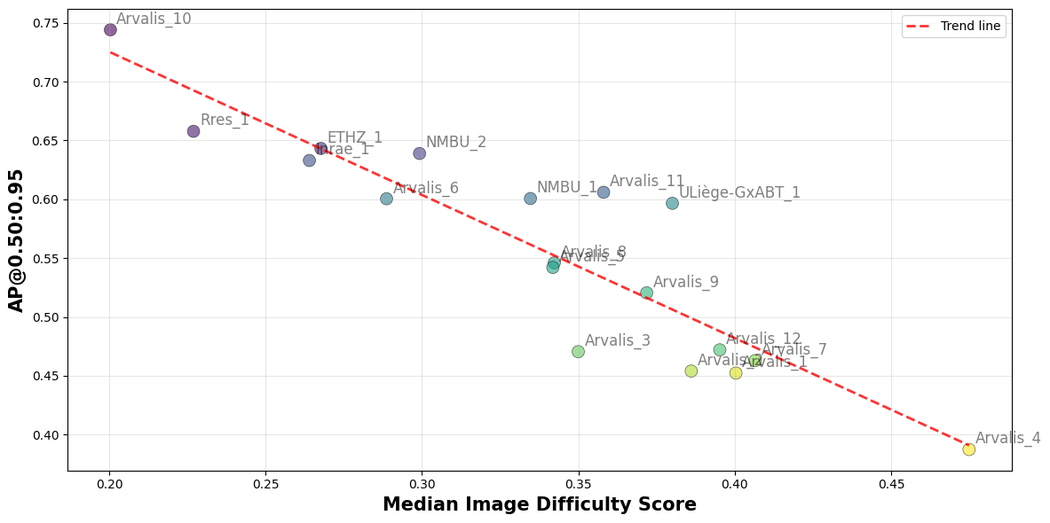
\includegraphics[width=\columnwidth]{gwhd_domain_score_satisfied.png}
  \caption{Domain/difficulty score visualization. Image converted to RGB, resampled to 1050\,px (3.5 in at 300 DPI) to comply with common IEEE figure requirements for single-column width.}
  \label{fig:score}
\end{figure}
\section{Discussion}
The diagnostic shows that although tiny objects have very low AP, their small share in the dataset limits potential absolute gains from focusing only on them. When MIS indicates a resolution ceiling, next steps should prioritize methods that increase effective information (e.g., super-resolution, domain-conditioned synthesis) rather than simple pixel duplication.
\section{Conclusion}
MIS is a compact, reproducible check to decide whether selection-based augmentation is likely to help. We release the notebook and the compliant figure in the repository.
\bibliographystyle{IEEEtran}
\bibliography{references}
\end{document}
